\subsection{Fravælgelse af gestik-par}
\label{TestresultaterVolumenDaarlig}
%
I følgende afsnit analyseres hvilke af de ni semaforiske gestik-par testpersonerne fravælger samt hvorfor testpersonerne netop fravælger disse gestik-par. På baggrund af analysen bør det være muligt at udpege hvilke semaforiske gestikker, der hvertfald ikke skal knyttes til at skrue op og ned for musikken. Analysen bygger på testpersonerne respons til spørgsmålet: \textit{Hvilken gestik kan du mindst lide? og hvorfor?}, hvor testpersonernes samlede data er vedlagt i ELEKTRONISK BILAG.
%
\begin{figure}[H]
	\centering
	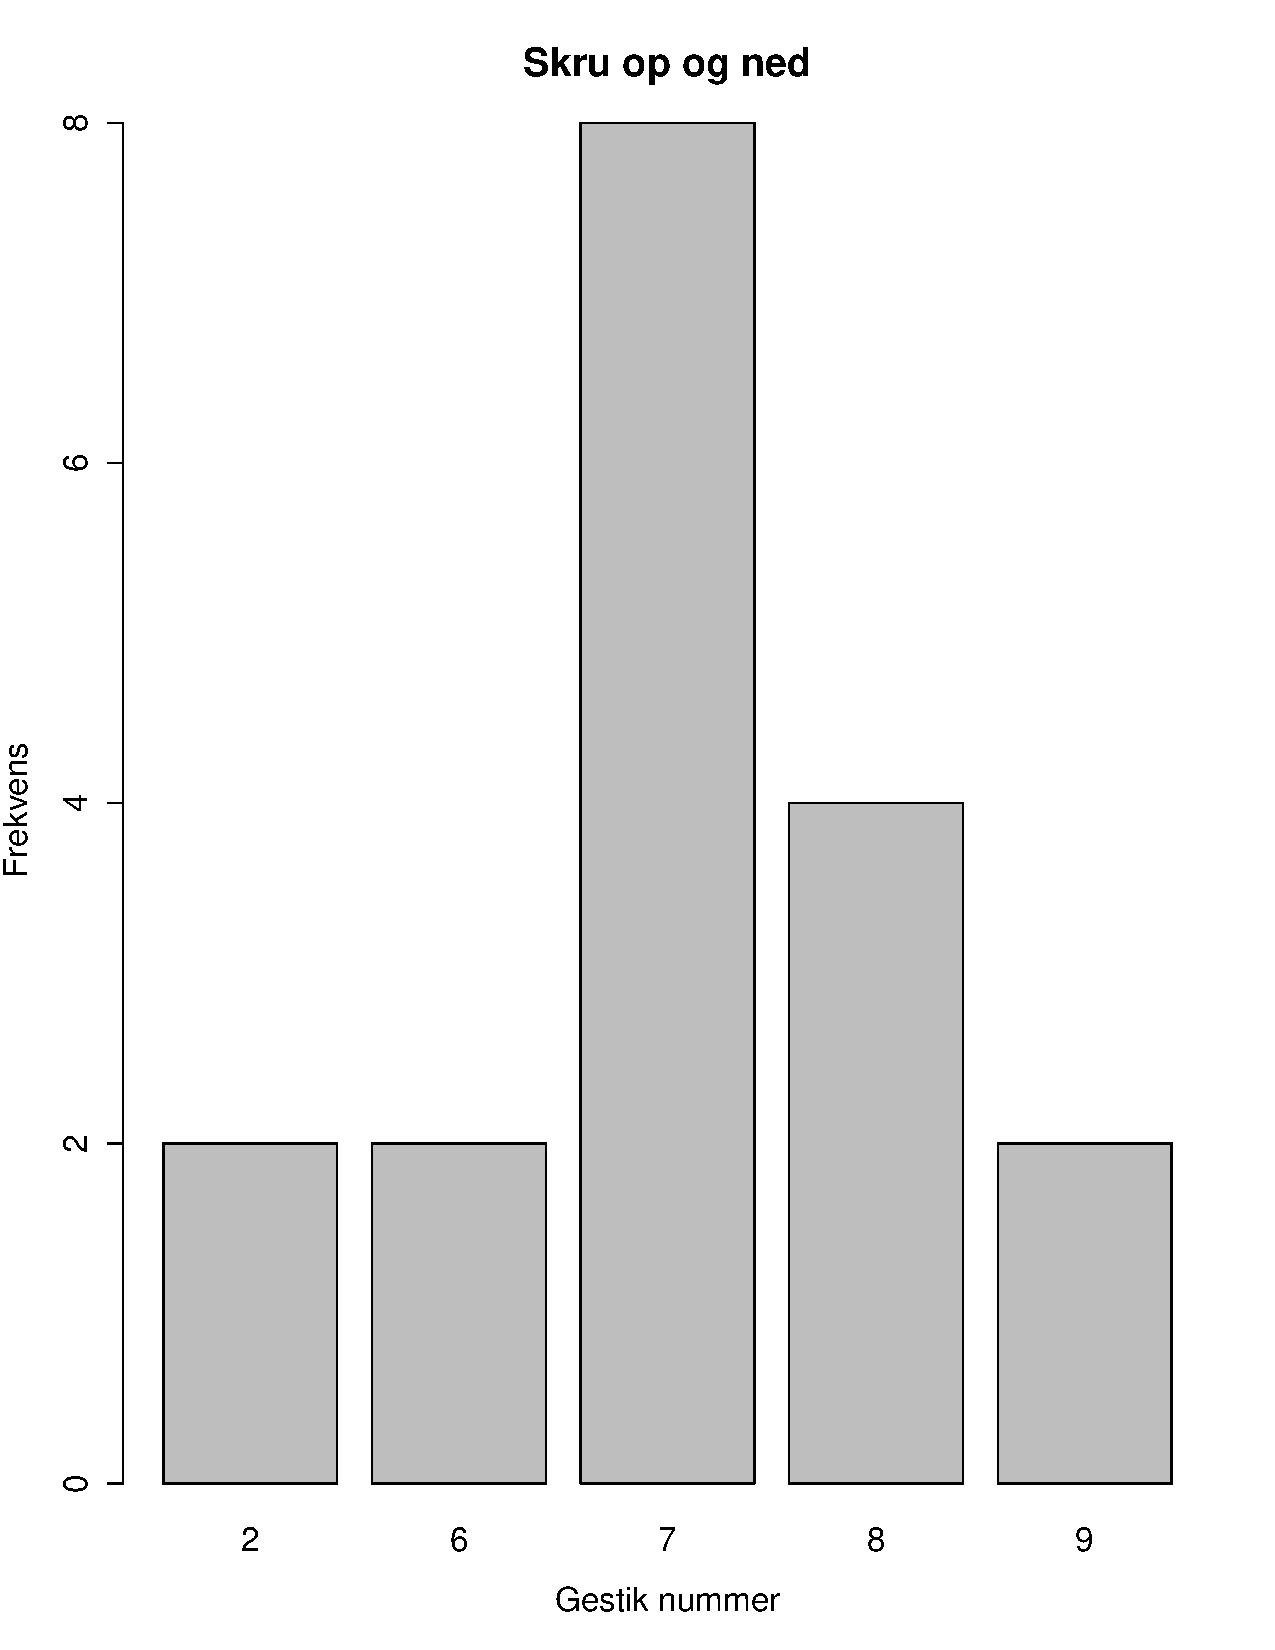
\includegraphics[resolution=300,width=0.5\textwidth]{Test1/DatabehandlingGrafer/DaarligstGestikVolumen.pdf}
	\caption{Barplot over hvilke gestik-par testpersonerne fravælger i forbindelse med at skrue op og ned for musikken. Søjlerne bygger på testpersonernes respons, hvorfor det kun er de fravalgte gestik-par, der udgør plottet.}
	\label{fig:DaarligstGestikVolumen}
\end{figure}
\noindent
%
På \autoref{fig:DaarligstGestikVolumen} fremgår det hvilke gestik-par de 18 testpersoner fravælger i forbindelse med at skrue op og ned for musikken. Det fremgår tydeligt at testpersonerne hyppigst fravælger gestik-par 7, parret er i alt fravalgt otte gange, og indgår ikke på en eneste top tre rangering (henvisning til en tabel jeg laver om lidt). Årsagen til at gestik-par 7 fravælges varierer mellem de otte testpersonerne, som har valgt parret. Testperson 2 har svært ved at vurdere hvilken vej der er op og hvilken vej der er ned. Ifølge testperson 3 er gestik-par 7 underligt og derudover så giver den ikke mening. At gestik-parret ikke giver mening pointere testperson 15 også og tilføjer, at det er en mellem ting mellem gestik-par 5 og gestik-par 6. Testperson 4 fravælger gestikken fordi den er mærkelig, hvilket også er en af årsagerne til at testperson 11 fravælger parret. Derudover kommenterer testperson 11 at det kræver koncentration at lave en bue, hvilket er en del af bevægelsen. Da formålet med at anvende semaforiske gestikker til at interagere med Bang $\&$ Olufsen's fremtidige musikanlæg, blandt andet er for at interaktionen på sigt kan foregå i den perifere opmærksomhed, så er det ikke hensigtsmæssigt at gestikkerne kræver mere koncentration end andre løsninger. Derudover påpeger testperson 10 at gestik-par 7 er væsentligt mindre intuitiv end de andre forslag og dertil er det svært at vurdere den nødvendige bevægelsesmængde for at skrue op og ned. Ifølge testperson 6 så er gestik-par 7 det par, som skiller sig mest ud i forhold til de andre forslag, hvilket er årsagen til at parret fravælges. Testperson 14's respons afvigere fra de andre testpersoners, i det at testperson 14 fravælger gestik-par 7 fordi testpersonen anser det som værende en meget naturlig bevægelse, som testpersonen giver udtryk for at ville komme til at lave ubevidst.

Selvom gestik-par 7 blev inkluderet som et forsøg på at overfører gestikken, der anvendes til at skrue op og ned på en A9, \parencite{WEB:BeoplayA9}, til en semaforisk gestik, så er gestik-par 7 det par, som oftes fravælges og som ikke indgår i nogen af testpersonernes top tre, hvorfor parret ekskluderes.\blankline
%
To ud af de fire testpersoner, som fravælger gestik-par 8, giver udtryk for at det er besværligt at pege nedad. Den ene af de to, testperson 18, giver stærkt udtryk for at det er både besværligt og ubehagligt at pege nedad samt at have sin arm i den position. Hvor den anden af de to testpersoner, testperson 9, giver udtryk for at det besværligt at brug og det er underligt at pege nedad. Derudover pointere testperson 9 at det er svært at kontrollere hvor meget der enten skal skrues og eller ned, hvilket også er årsagen til at testperson 5 fravælger gestik-par 8; der er ingen mulighed for at kontrollere hvor meget der skrues op. Den sidste af de fire testpersoner, testperson 13, fravælger gestik-par 8 fordi der mangler bevægelse og fordi det er noget testpersonen godt kunne forestille sig komme til at gøre ved et uheld.  

Der er to forskellige årsager til hvorfor gestik-par 2 fravælges af testperson 12 og testperson 16. Testperson 12 fravælger gestik-par 2 fordi testpersonen ikke bryder sig om cirkelbevægelsen, selvom testpersonen pointere at det burde virke naturligt og det egentlig er sådan der normaltvist skrues op på et anlæg. Det skal dog pointeres at testperson 12 ikke endegyldigt fastslår at det er gestik-par 2, da testpersonen egentlig heller ikke bryder sig om gestik-par 1. Grunden til at det fremgår, som om at testperson 12 har valgt gestik-par 2 er på baggrund af de bevægelser, der opstår når testpersonen skal forklare hvorfor der vælges som der gør og i det tilfælde stemte bevægelsen overens med bevægelsen i gestik-par 2. Den årsager til at gestik-par 2 fravælges er fordi bevægelsen, ifølge testperson 16, er modsat af hvad testpersonen ville forvente. Det skal dog pointeres at der ved gestik-par 2 skrues op for musikken ved at dreje hånden med uret og mod uret for at skrue ned, hvilket er det testpersonen egentlig forventer. Det tyder derfor på at testperson 16 har misforstået videooptagelsen af gestik-par 2. Testlederen spørger derfor ind til hvordan gestik-par 2 kunne gøres bedre, hvor testperson 16 først og fremmest foreslår at bevægelsen foregår i den rigtige retning og derudover foreslår testpersonen at gestikken skulle være mere ligesom gestik-par 1, hvor testpersonen referer til armens position.  

Gestik-par 6 fravælges af testperson 9 fordi det vil være svært at gengive bevægelsen med et barn på armen, hvilket også gør sig gældende for gestik-par 5. Testperson 17 fravælger gestik-par 6 fordi det er ulogisk at lave den bevægelse i forbindelse med musik og derudover virker det mærkelig at begge hænder skal være involveret. 

Ifølge testperson 7 så fravælges gestik-par 9 fordi den ikke tillader kontrol over hvor meget der skrues op og ned, hvorimod testperson 8 fravælger gestik-par 7 fordi testpersonen vil have det akavet med at lave den bevægelse.
%
\begin{table}[H]
	\centering
	\begin{tabular}{ | p{1.5cm} | p{2.1cm} | p{2.1cm} | p{2.1cm} | p{2.1cm} | p{2.1cm} |}
	\hline
		 & Gestik-par 2 & Gestik-par 6 & Gestik-par 7 & Gestik-par 8 & Gestik-par 9 \\ \hline
		1. Plads & 4 & 1 & 0 & 0 & 2\\ \hline
		2. Plads & 2 & 2 & 0 & 0 & 1\\ \hline
		3. Plads & 3 & 1 & 0 & 2 & 3\\ \hline
	\end{tabular}
	\caption{Oversigt over hvor ofte og hvor de fem fravalgte gestikker indgår i testpersonernes top tre rangering.}
	\label{tab:FravalgteTopTreVolumen}
\end{table}
\noindent
%
På baggrund af \autoref{tab:FravalgteTopTreVolumen} sammenholdt med \autoref{fig:DaarligstGestikVolumen} samt testpersonernes begrundelser, tyder det på, at der er belæg for at ekskludere gestik-par 8 fra fremtidige undersøgelser. Selvom det ikke kan antages med sikkerhed at testperson 16 ville have udpeget et andet gestik-par, i tilfælde af at testpersonen ikke havde misforstået bevægelsesretningen i gestik-par 2, så tyder det på, at det godt kunne være tilfældet. I så fald, så er det kun testperson 12, som har givet udtryk for at en cirkulærbevægelse ikke foretrækkes. Da det heller ikke entydigt kan konkluderes hvorvidt testperson 12 mindst kan lide gestik-par 2 i forhold til gestik-par 1 og da gestik-par 2 sammenlagt indgår ni gange i testpersonernes top tre, jævnfør \autoref{tab:FravalgteTopTreVolumen}, vurderes det at der ikke er belæg for at ekskludere gestik-par 2. 

For at have belæg for at ekskludere gestik-par 6 er det nødvendigt at inkludere hvad testpersonerne, som har rangeret gestik-par 6 i deres top tre, har kommenteret. Ifølge testperson 1 så indgår gestik-par 6 på en anden plads dels fordi den følger et princip om noget der er større eller mindre og dels fordi bevægelsen er naturlig. Det tyder på at testperson 14 rangere gestikker alt efter hvad der føles akavede og unaturligt i frygt for at komme til at lave gestikkerne ved et uheld, hvilket er årsagen til at testperson 14 har tildelt gestik-par 6 en anden plads. Testperson 2 forklarer at årsagen til at gestik-par 6 rangeres på en tredje plads, er fordi den minder om gestik-par 4 og gestik-par 5 bare sidelæns, men at det ikke giver lige så meget mening, som de to andre. Baseret på testperson 5's udsagn tyder det på at årsagen til at gestik-par 6 tildeles en første plads er fordi testpersonen ønsker at have fuld kontrol over hvor meget der skrues op og ned, hvilket testpersonen oplever ved at bruge begge hænder. Grunden til at testpersonen vælger gestik-par 6 fremfor gestik-par 5 skyldes, at testpersonen derved føler sig mindre i rummet.      

TJEK HVAD DE GØR TIL 6'EREN






